\documentclass[a4paper,11pt]{article}

% Import packages
\usepackage[a4paper]{geometry}
\usepackage[utf8]{inputenc}
\usepackage{amsmath}
\usepackage{amssymb}
\usepackage{graphicx}

\graphicspath{ {images/} }
\DeclareGraphicsExtensions{.pdf,.jpeg,.png,.jpg}

% Change enumerate environments you use letters
\renewcommand{\theenumi}{\alph{enumi}}

% Set title, author name and date
\title{Foursum Report}
\author{Elias Jørgensen, Simon Høiberg}
\date{\today}

\begin{document}

\maketitle

\section*{Exhaustive search}

\ \ \ \
Our program [Simple.java] solve the Four-sum problem using $ 4 $ nested loops. \\
The index variables \textit{i, j, k, l} are initialized and run from loop $ 1, 2, 3, 4 $,
respectivly, and are all used in a conditional statement within the most inner loop no. 4. \\
We can bound the number of array accesses by $\sim N^4 $ in worst case.

\section*{Experiments}

\ \ \ \
The following table summarizes the empirical performance data on the input files in the data directory.\\
We have run each file once, and report the minimum, maximum and average running time over the files
for each input size. \\
\hspace{5mm}\\

{
\centering
\begin{tabular}{cccc}
\hline
\textit{N} & \textit{Min} & \textit{Max} & \textit{Avg} \\
\hline
100 & 0.007 s & 0.01 s & 0.0086 s \\
200 & 0.091 s & 0.097 s & 0.093 s \\
400 & 0.799 s & 1.408 s & 1.207 s \\
800 & 11.59 s & 19.49 s & 17.84 s \\
1600 & 4:30 m & 8:37 m & 5:30 m \\
3200 & 3:50 m & 1:15 h & 1:00 h \\
\hline
\end{tabular}
\quad
\begin{tabular}{cccc}
\hline
\textit{N} & \textit{Min} & \textit{Max} & \textit{Avg} \\
\hline
100 & 2.585 s & 2.995 s & 2.79 s \\
200 & 34.981 s & 41.763 s & 38.372 s \\
400 & 6:29 m & 6:54 m & 6:42 m \\
\hline
\\
\\
\\
\end{tabular}\\
}

\hspace{5mm}\\
\hspace{5mm}\\

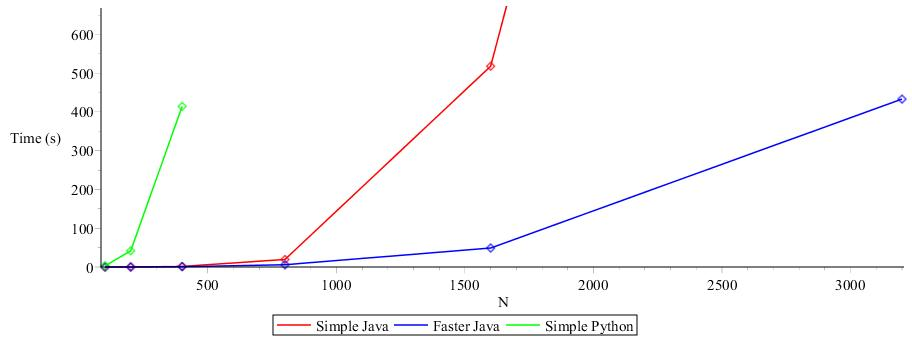
\includegraphics[width=380px]{simple-plot}

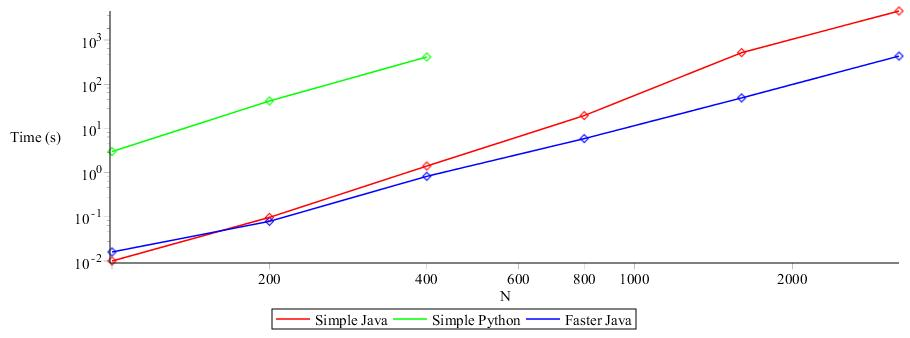
\includegraphics[width=380px]{simple-plot-log}\\
\hspace{5mm}\\

\section*{Improvements}
Using the binary search-based idea sketeched in [SW, 1.4] for the
Three-sum problem, we can improve our running time to $\sim N^3 \log N $. \\
The following table reports our the minimum, maximum and average running time
on the test inputs from the files in the data directory. \\
\hspace{5mm}\\

\centering
{
\begin{tabular}{cccc}
\hline
\textit{N} & \textit{Min} & \textit{Max} & \textit{Avg} \\
\hline
100 & 0.0 s & 0.016 s & 0.0094 s \\
200 & 0.031 s & 0.079 s & 0.0665 s \\
400 & 0.297 s & 0.824 s & 0.6424 s \\
800 & 2.45 s & 5.875 s & 5.0668 s \\
1600 & 18.38 s & 48.953 s & 42.69 s \\
3200 & 2:44 m & 7:13 m & 6:13 m \\
\hline
\end{tabular}
}

\end{document}
